\scanpage{114}
% archive foliation: 115
Cristaux de Modules \{loc. libres\} $=$ Modules loc. libres sur le site cristallin

\uline{Ex. 1}\quad $S$ \deleted{schéma} \inserted{$=\operatorname{Spec}A_o$, $A_o$ anneau} parfait de car $p>0$.

$A=W(A_o)$, alors les cristaux sur $A_o$ sont les Modules loc. libres sur $A$

\uline{Ex. 2}\quad $X_o$ lisse sur corps parfait $k$, $W=W(k)$,
$\mathfrak X$ remontant $X_o$ en schéma \inserted{formel} lisse sur $W$,
\deleted{[\unsure{et} $F:X-X$ remontant \unsure{Frobenius} en un hom $\unsure{\sigma_W|\varphi_W}$-linéaire de $X$]}
Un cristal est un module loc. libre $M$ sur $\mathfrak X$, muni connexion à courbure nulle rel/$W$.

Ce sont des \unsure{genres|germes} d'animaux \deleted{\unsure{dans}} rencontrés anciennement par Dwork, Katz, $\ldots$
\deleted{\unsure{Monsky}}

\figure{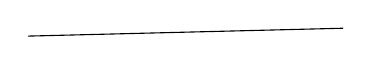
\begin{tikzpicture}\draw(0,0)--(4,.1);\end{tikzpicture}}
4)

I) $S$ schéma avec $p$ loc nilpotent. On définit ``foncteur de Dieudonné''
\[
\mathrm{BT}(S)^o\longrightarrow\mathrm{Cris}\,\mathrm{mod}\,\mathrm{loclib}(S)
\]
\[
G\longmapsto\mathbf D(G)
\]
\margin{compatible aux chgt. de base}

II) \deleted{Soit} $S$ de car. $p$, alors $M=\mathbf D(G)$ est muni de $F_M,V_M$ avec
\[
F_MV_M=p.\operatorname{id},\qquad V_MF_M=p\operatorname{id}
\]
i.e. $D(G)$ est un cristal de Dieudonné.

Il se pourrait que le foncteur \unsure{!}
\[
\mathrm{BT}(S)^o\longrightarrow\mathrm{Cris}\,\mathrm{Dieud}(S)
\]
soit pl. fidèle, et j'ai une idée de ce qui pourrait être l'image essentielle
